\documentclass[portrait,color=UCLblack,margin=1.5cm,bannerheight=8cm,logoheight=2.5cm]{uclposter}
\usepackage{tikz}
\usepackage[scaled=1.2]{helvet}
\renewcommand\familydefault{\sfdefault} 
\usepackage[T1]{fontenc}
\usepackage{tcolorbox}

\title{Performance characterisation of 8-bit RISC and OISC architectures}

\author{Mindaugas Jarmolovicius}

%\affil[1]{UCL Electronic And Electrical Engineering}

\begin{document}

%\tikz\node[opacity=0.3,inner sep=0]{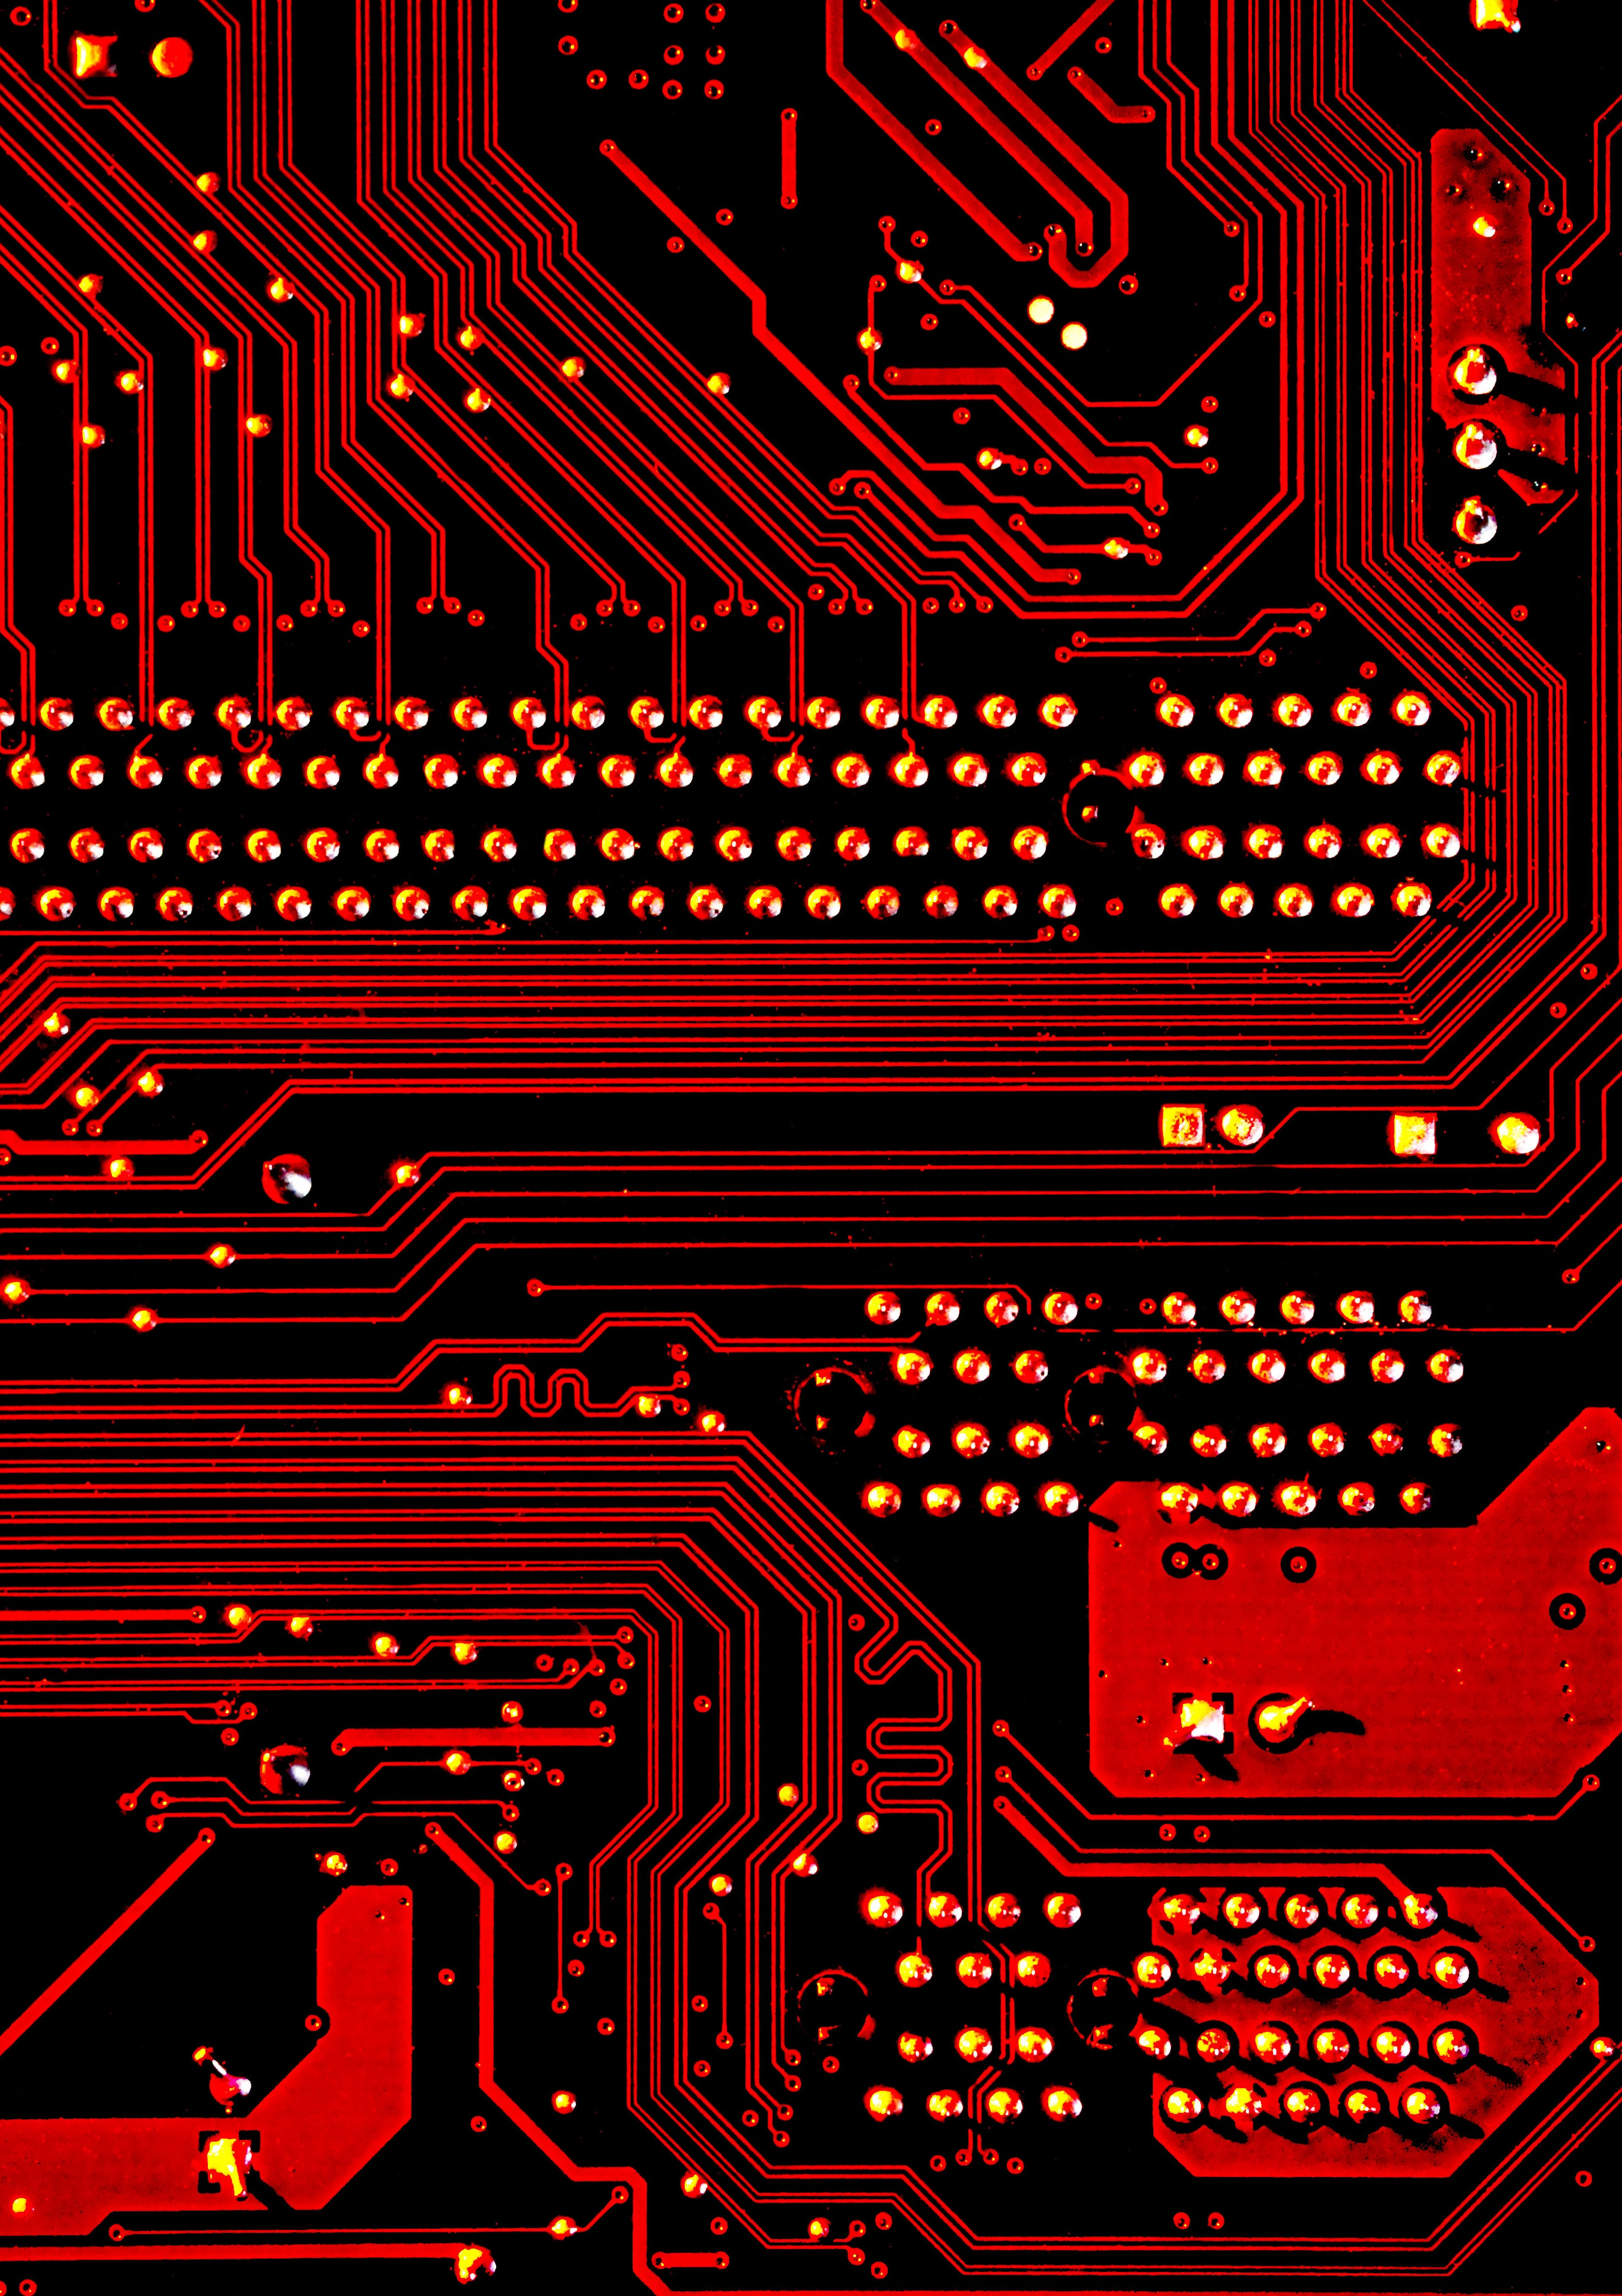
\includegraphics[height=\paperheight,width=\paperwidth]{background.jpg}}
%\tikz[remember picture,overlay] \node[opacity=0.3,outer sep=0pt] at (current page.center){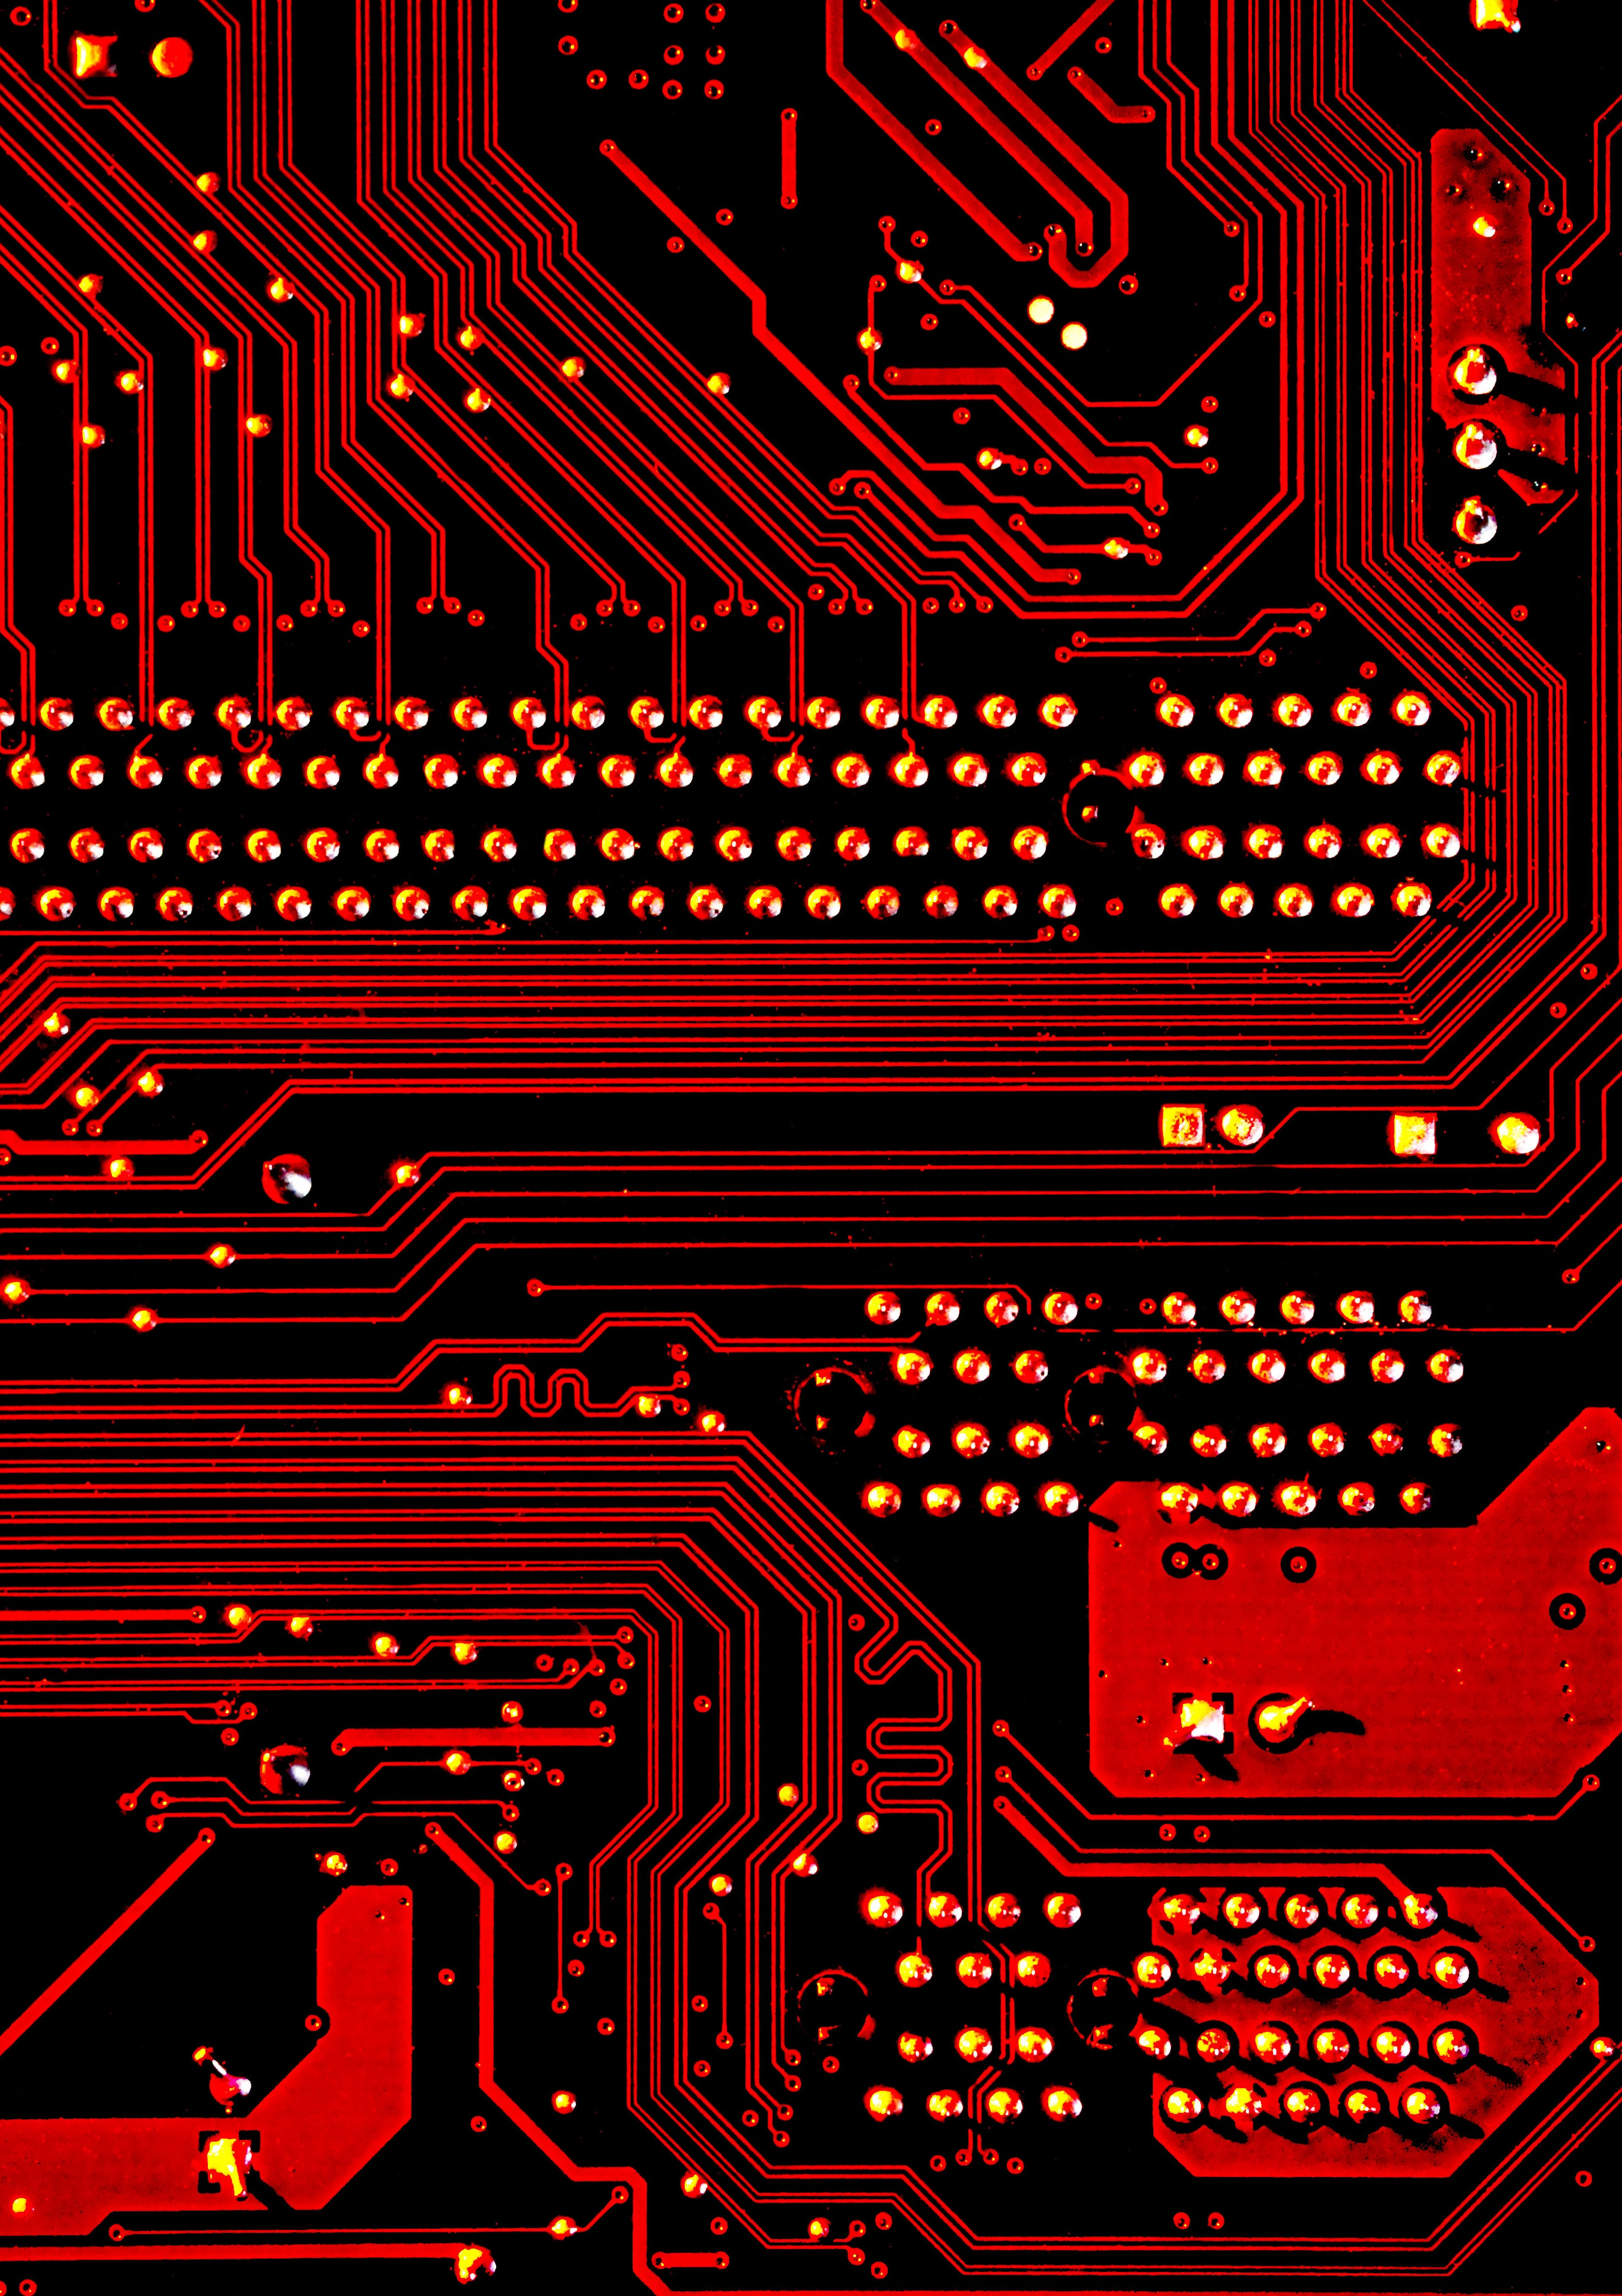
\includegraphics[width=\paperwidth,height=\paperheight]{background.jpg}};

\maketitle

\begin{tcolorbox}[title=\large{Introduction}]
	
This is a bunch of text for introductions that describes project, what it is about and that it compares RISC versus OISC architectures.
\end{tcolorbox}


\begin{multicols}{2}
	
\begin{tcolorbox}[title=\large{OISC}]
	\begin{description}
		\item[$\bullet$] Bunch of instructions
		\item[$\bullet$] Efficient instruction space
		\item[$\bullet$] Generally easy to use but damn to low number of registers.
		\item[$\bullet$] Needs optimisation.
	\end{description}
\end{tcolorbox}

%\begin{highlightbox}[UCLdarkblue!20!white]
%\end{highlightbox}

\columnbreak


\begin{tcolorbox}[title=\large{OISC}]
	OISC is fun. Some graphs here.
	\begin{description}
		\item[$\bullet$] Only one instruction
		\item[$\bullet$] Not so efficient instruction space
		\item[$\bullet$] Takes forever to write in assembly
		\item[$\bullet$] Takes no time to improve. It just asking for more data buses!
	\end{description}

\end{tcolorbox}

\end{multicols}

\section*{Results}
This is section with some results if I will have enough time to complete them.. \textbf{RIP MY FREE TIME}.

\section*{Future work}
Explain future work, experiments, oisc improvements.


\end{document}
